\documentclass[journal]{IEEEtran}
\usepackage[a5paper, margin=10mm, onecolumn]{geometry}
\usepackage{cite}
\usepackage{amsmath,amssymb,amsfonts,amsthm}
\usepackage{algorithmic}
\usepackage{graphicx}
\usepackage{textcomp}
\usepackage{xcolor}
\usepackage{txfonts}
\usepackage{enumitem}
\usepackage{mathtools}
\usepackage{gensymb}
\usepackage{comment}
\usepackage[breaklinks=true]{hyperref}
\usepackage{tkz-euclide}
\usepackage[latin1]{inputenc}                                
\usepackage{color}                                            
\usepackage{array}                                            
\usepackage{longtable}                                       
\usepackage{calc}                                             
\usepackage{multirow}                                         
\usepackage{hhline}                                           
\usepackage{ifthen}                                           
\usepackage{lscape}

\setlength{\headheight}{1cm} % Set the height of the header box
\setlength{\headsep}{0mm}     % Set the distance between the header box and the top of the text

\begin{document}

\bibliographystyle{IEEEtran}
\setlength{\intextsep}{10pt} % Space between text and floats
\numberwithin{equation}{section} % Use section numbering for equations
\numberwithin{figure}{section} % Use section numbering for figures
\numberwithin{table}{section} % Use section numbering for tables

\title{9-9.2-13}
\author{AI24BTECH11016 - Jakkula Adishesh Balaji}
\maketitle
\section*{\textbf{Intersection Of Conics(Chords)}}
\parindent 0pt
\textbf{Question:} \\
\textbf{9.2.13} Find the area of the region bounded by the ellipse $\frac{x^{2}}{16} + \frac{y^{2}}{9} = 1$\\
\solution
Equation of curve in Matrix form is \\
\begin{align}
\vec{x}^\top\vec{V}\vec{x} + 2\vec{u}^\top\vec{x} + f = 0
\end{align}
For the given ellipse, The values of $\vec{V}$,$\vec{u}$,$f$ are
\begin{align}
\vec{V}&=\begin{pmatrix}9 & 0\\0 & 16\end{pmatrix}\\
\vec{u}&=\begin{pmatrix}0\\0\\\end{pmatrix} \\
f&=-144
\end{align}
The area under the curve is given by \\
\begin{align}
A &= 4 \int_0^4 3 \sqrt{1 - \frac{x^2}{16}} \, dx \\
A &= 12\pi 
\end{align}
\begin{table}[h!]    	
    \centering
    % Assuming the table.tex file exists
    \begin{tabular}[12pt]{ |c| c|}
    \hline
    Parameter & Description\\ 
    \hline
    $P$ & $\myvec{2\\-3}$ \\
    \hline 
    $Q$ & $\myvec{10\\y}$ \\
    \hline
    $D$ & $Q-P$\\
    \hline 
    Distance & $10$ \\
    \hline
    \end{tabular}
 
    \caption{Parameters Used}
    \label{tab:1-1.9-6}
\end{table}
\begin{figure}[h!]
    \centering
    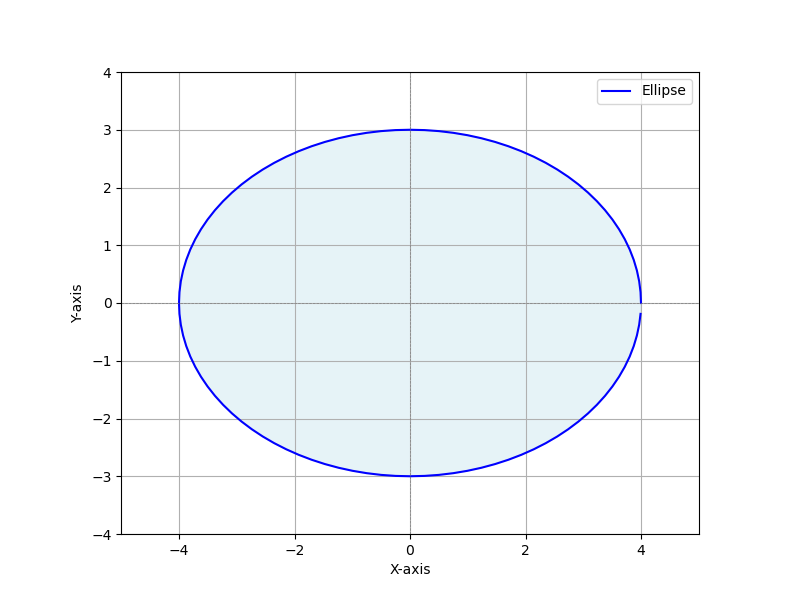
\includegraphics[width = 1\linewidth]{figs/Figure_1.png}
    \caption{Plot of ellipse}
    \label{fig:stemplot}
\end{figure}
\end{document}


